% !TeX spellcheck = ru_RU
% !TEX root=../main.tex

\begin{lecture}[Методы решения уравнений процессов]
	\begin{lecSection}[Введение]
	Есть переменные $ N, V $ и параметры $ F_1 (\vec{R_1}), F_2 (\vec{R_2}), \dots, F_n (\vec{R_n}) $. 
	
	\begin{figure}
	\begin{minipage}{0.48\linewidth}
%		\begin{figure}
		\centering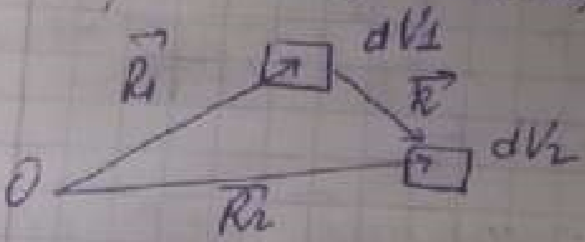
\includegraphics[width=\linewidth]{lecture_12/scheme1}
		\label{fig:12:scheme1}
		\caption{К выводу}
	\end{minipage}
	\begin{minipage}{0.48\linewidth}
		\begin{gather*}
			d P \left( \vec { R } _ { 1 } , \vec { R } _ { 2 } \right) =
			F _ { 2 } \left( \vec { R } , \vec { R } _ { 1 } \right) \frac { d V _ { 1 } } { V } \frac{dV_2}{V} = \\
			= F_2 \left( \left| \vec{R_2} \vec{R_1} \right| \right) \frac{dV_1 dV_2}{V^2} = F_2 (R_{12}) \frac{dV_1 dV_2}{r^2} \\
			F_2 ( f_R ) \equiv g (R)
		\end{gather*}
	\end{minipage}
	\end{figure}
	
	\begin{center}\begin{tabular}{cc}
		\multicolumn{2}{c}{RDF} \\
		$ dV = 4 \pi R^2 dR $ & $ d P_{12} = \frac{dV_1}{V} \frac{dV_2}{V} $ \\
		\multicolumn{2}{c}{$ g (R) \rightarrow 1\, \text{при } R \rightarrow \infty;\, R \rightarrow 0\,~~ g(R) = 0, \, 0 \leq R < 2r $} \\
	\end{tabular}\end{center}
	\begin{gather*}
	\int\limits_\text{объему} dn = \int \rho ( R ) \cdot 4 \pi R ^ { 2 } d R = N - 1, ~~ N >> 1 \\
	\left.\begin{array}{c}
	\dfrac{1}{N} \displaystyle \int\limits_0^\infty 4 \pi R^2 \rho (R) dR = 1 \\
	\dfrac { 1 } { V } \displaystyle \int\limits_0^\infty g ( R ) 4 \pi R ^ { 2 } d R = 1
	\end{array} \right \}
	\begin{array}{c}
		\dfrac{g (R)}{V} = \dfrac{\rho (R)}{N} \\
		\dfrac{N}{V} = \rho_0 \\
		\boxed{ \rho(R) = g(R) \rho_0 } \\
		g(R) \text{ --- рад. функция} \\ \text{распределения}
	\end{array}
	\end{gather*}
	\underline{Пример}: $ u(R),~ u=? \tab u = \dfrac{3}{2}\, kTN + \dfrac{1}{2}\, N \rho_0 \displaystyle \int\limits_0^\infty u(R) g(R) \cdot 4\pi R^2 dR $
%	\begin{lecSection}[Идеальный газ]
%		TODO: pic
		\begin{figure}[h]
		\begin{minipage}{0.35\linewidth}
			\centering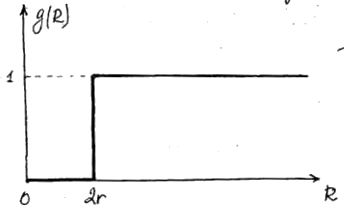
\includegraphics[width=\linewidth]{lecture_12/new_id_gas1}
			\caption{Идеальный газ}
		\end{minipage}
		\begin{minipage}{0.28\linewidth}
			\centering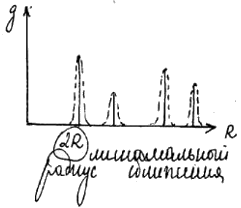
\includegraphics[width=\linewidth]{lecture_12/new_id_gas2}
			\caption{Кристаллическая фаза}
		\end{minipage}
		\begin{minipage}{0.35\linewidth}
			\centering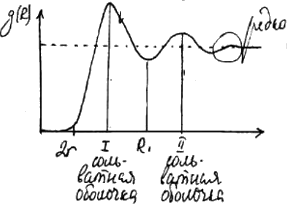
\includegraphics[width=\linewidth]{lecture_12/new_id_gas3}
			\caption{Жидкая фаза}
			\label{fig:12:liq_scheme}
		\end{minipage}
	\end{figure}

	На рис. \ref{fig:12:liq_scheme} выделено количество частиц в одной сольватированной оболочке, равное $ S $.

	\begin{gather*}
		Li^+ \tab n = 5 - 24~ \text{количество ионов в одной сольватной оболочке} \\
		n_1 = 4 \pi \rho_0 \displaystyle \int\limits_0^{r_1} g(r) r^2 dr \\
		n_2 = 4 \pi \rho_0 \displaystyle \int\limits_{r_1}^{r_2} g(r) r^2 dr
	\end{gather*}
	\begin{minipage}{0.3\linewidth}
		\centering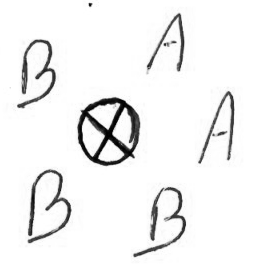
\includegraphics[width=0.6\linewidth]{lecture_12/id_gas4}
	\end{minipage}
	\begin{minipage}{0.3\linewidth}
		$ A/B ~~~~
			\begin{cases}
				\rho_A (R) = g_{AA} (R) \rho_{A0} \\
				\rho_B (R) = g_{AB} (R) \rho_{B0}
			\end{cases} $
	\end{minipage}
%	\end{lecSection}
	\end{lecSection}
	\begin{lecSection}[Метод квазистационарных концентраций \\ (метод Семенова-Боденштейна)]
		\begin{gather*}
			\frac { d A _ { 1 } } { d t } = - k _ { 1 } A _ { 1 } + \ldots \\
			\frac { d A_2 } { d t } = k_1 A_1 - k \ldots \\
			\frac { d p } { d t } = f \left( A_1 , \ldots , A _ { n } \right) \\
			l = O(1) \tab \begin{cases}
			\varepsilon = 0 \text{ невозмущенная} \\
			\varepsilon \neq 0 \text{ возмущенная}
			\end{cases}
		\end{gather*}
		
		\begin{center}\begin{tabular}{ll}
			\multicolumn{2}{c}{$ A \xrightarrow{k_1} B \xrightarrow{k_2} P $}  \\
			$ \dfrac { d A } { d t } = - k A, $ & $ A(0) = A_0, ~~ B(0) = 0 $ \\
			$ \dfrac { d B } { d t } = k A - k_2 B, $ & $ A_0 = A + B + P $ \\
			\multicolumn{2}{c}{$ x = \dfrac{B}{A_0}, ~ y = \dfrac{A}{A_0}, ~ r = k_1 t $}
		\end{tabular}\end{center}
		Здесь мы взяли в качестве характерного времени $ \tau = 1/k_1 $. При этом $ \varepsilon = k/k_2 $
		
		\begin{figure} % Чтобы работал \caption
		\begin{minipage}{0.48\linewidth}
			\centering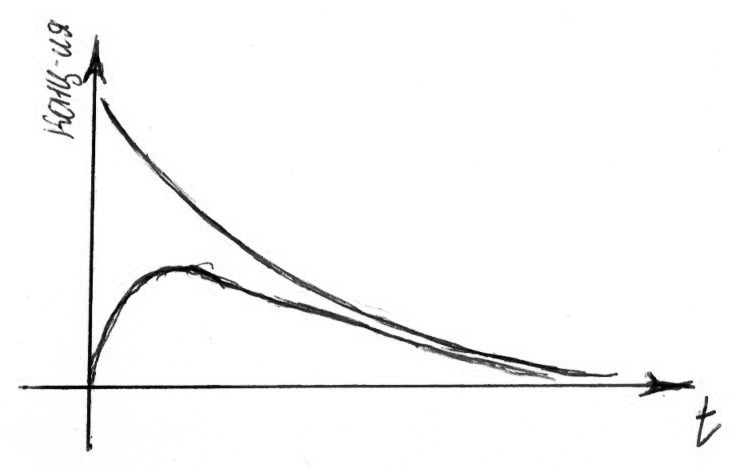
\includegraphics[width=\linewidth]{lecture_12/vozm1}
			\caption{Иллюстрация к методу возмущений}
			\label{fig:12:vozm_illustration}
		\end{minipage}
		\begin{minipage}{0.48\linewidth}
			\centering Метод возмущений:
			\begin{gather*}
				\begin{cases}
					\varepsilon \dot{x} = f (x, y) \\
					\dot{y} = g (x, y)
				\end{cases} \\
				\begin{cases}
					f(x, y) = 0 \\
					\dot{y} = g(x, y)
				\end{cases}
			\end{gather*}
		\end{minipage}
		\end{figure}
		\begin{gather*}
			\dot{x} = F(x, \varepsilon) \\
			\dot{x} = F(x, 0) \\
			x = \varphi (t, \varepsilon) \\
			\varphi (t, \varepsilon) = \varphi (t) + R_0 (t, \varepsilon) \\
			R_0 (t, \varepsilon) \xrightarrow[\varepsilon \rightarrow 0]{} 0 \\
			\varphi (t, \varepsilon) = \varphi_0 (t) + \varepsilon \varphi_1 (t) + \dots \varepsilon^\gamma \varphi_n (t) \\
			\dot{x} = \dfrac{1}{\varepsilon} f (x, y)
		\end{gather*}
	\end{lecSection}
\end{lecture}